\documentclass[notitlepage]{article}

\title{Northern Reaches}

\author{quajzen}

\date{Last updated \today}
\usepackage{accanthis}

\usepackage{graphicx}

\usepackage[margin=2cm]{geometry}

\usepackage{multicol}

\setlength{\columnsep}{1cm}

\usepackage{microtype}

\begin{document}
\maketitle
\vfill
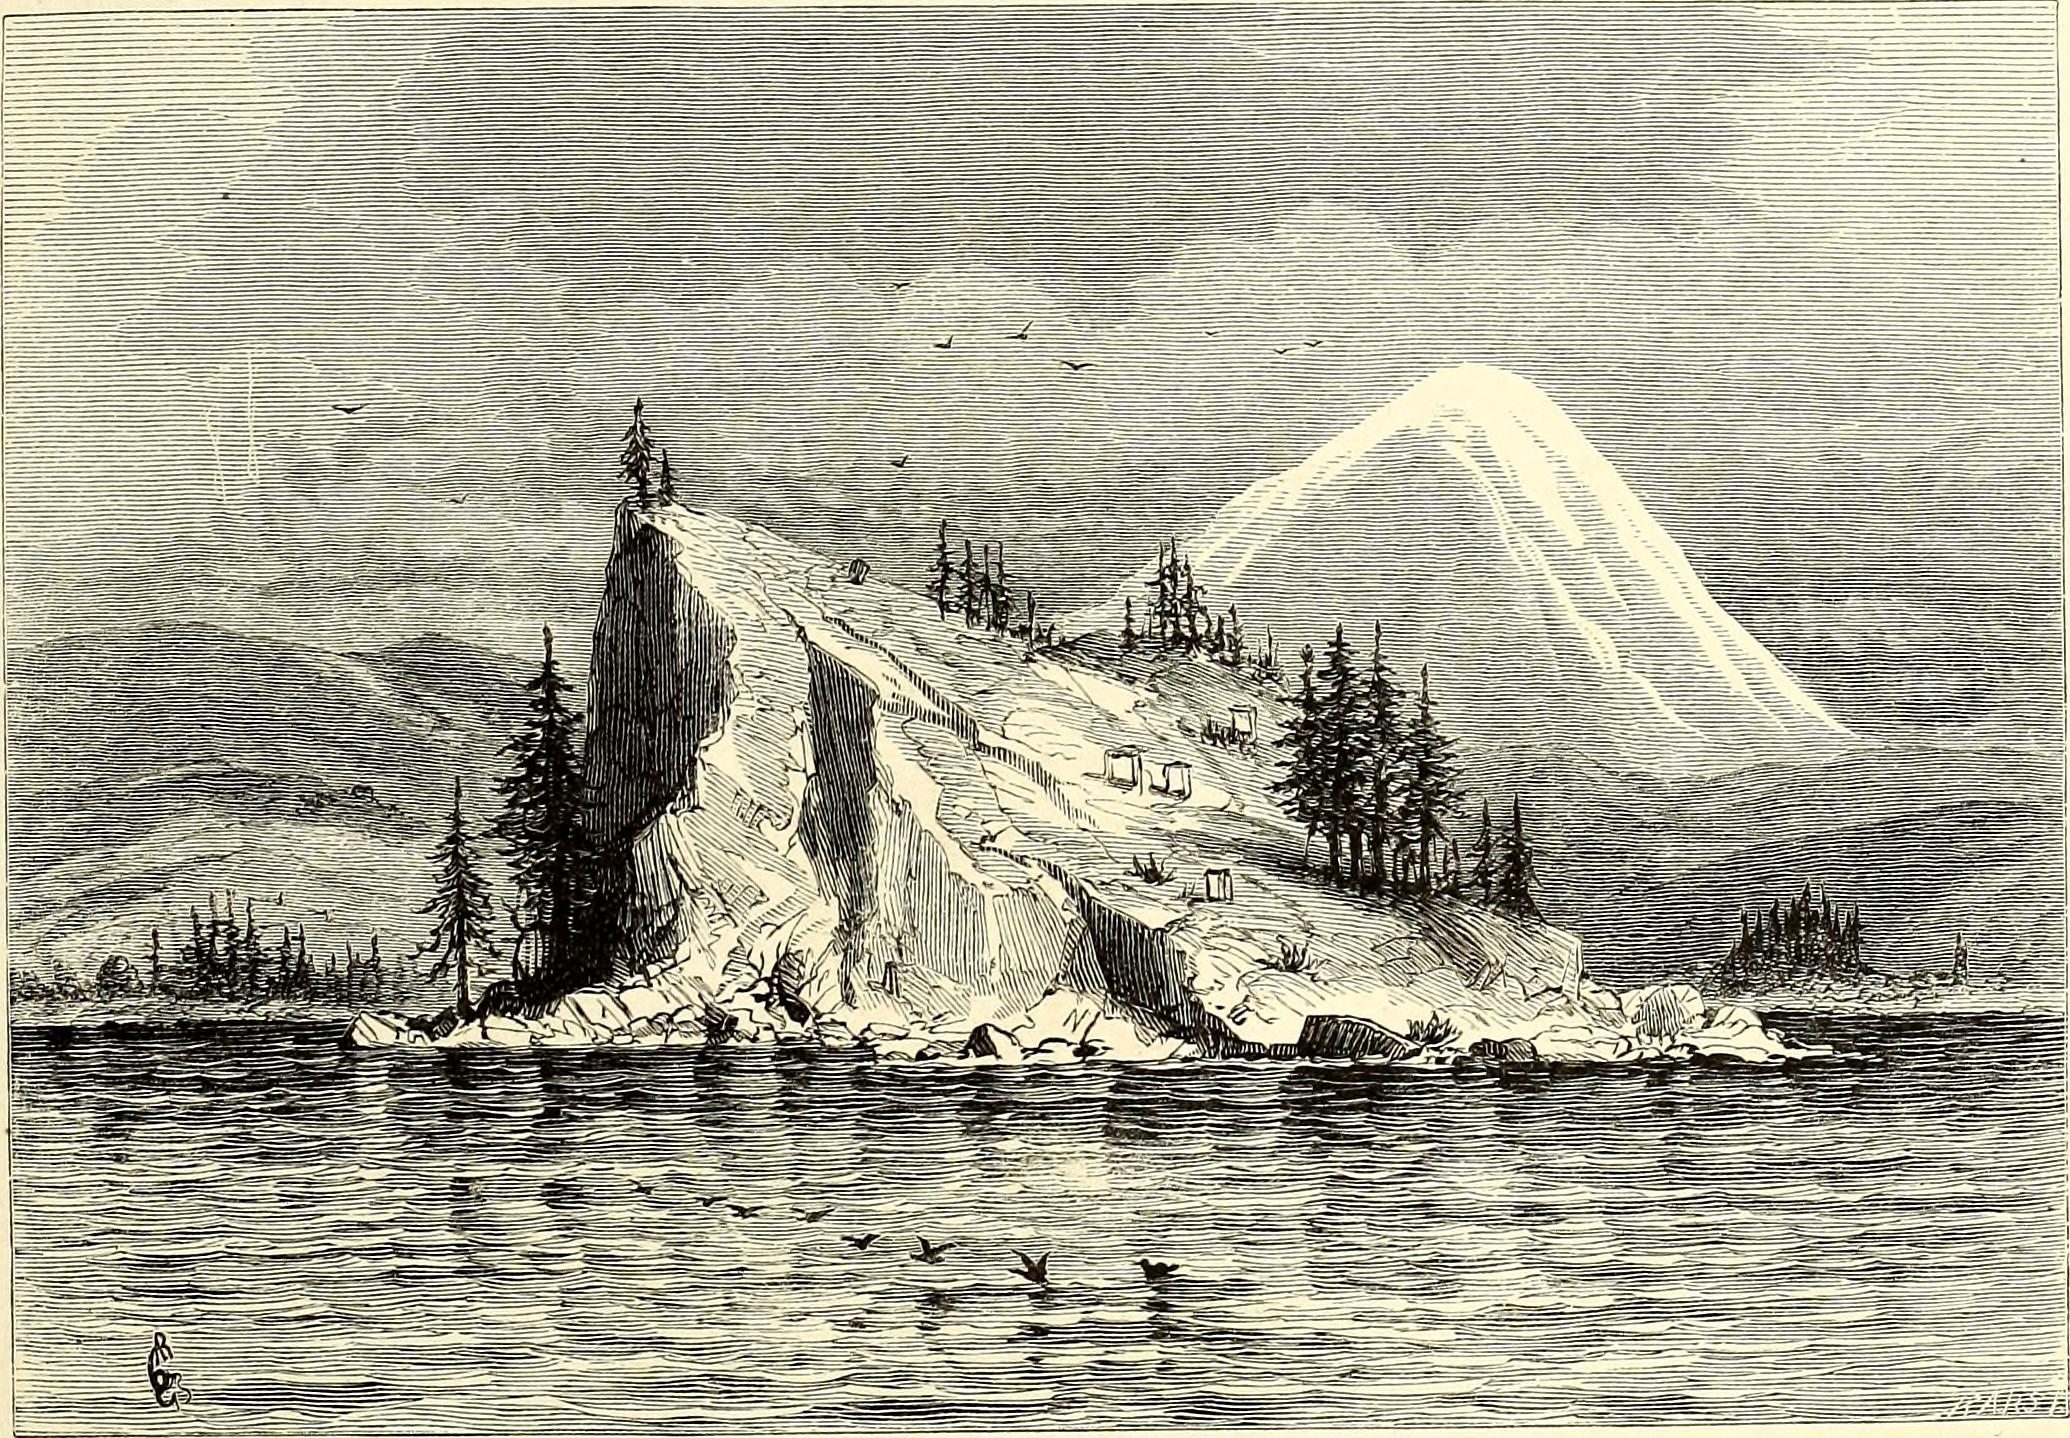
\includegraphics[width=\textwidth]{cover}
\newpage
\tableofcontents
\listoftables
\newpage

\begin{multicols}{2}
  
\section{Introduction}

This is a setting zine and toolkit for a far-north biome. This zine contains some basic overview of the setting and a playable adventure site.

\subsection*{What are the Northern Reaches?}

The Northern Reaches are the name for a region close to the poles of your world, one which is dominated by snowy and icy biomes: taiga, polar seas, and icy wastes. \\

It was once the realm of a great kingdom centuries ago, but a sudden onset of cold and ice quickly extinguished this society.
Now, however, the ice is slowly receding, revealing long-lost treasures. \\

The recession of the cold has allowed some settlers to come in and reclaim some of the land, some to settle more permanently and others looking to plunder this lost land. \\

They are not the only life out in the Reaches; many well--adapted creatures live in the wilderness outside of the settled towns.
The Reaches provide many natural resources for trade: lumber, ore, fish, and furs, but the living is tough.

\subsection*{Where are the Northern Reaches?}

You may use this setting as a stand-alone location, or incorporate it into a larger campaign world you have or will establish.
Use this setting in a cold polar region.

\subsection*{What Kind of World is the Northern Reaches In?}

Anything you like.
A fitting world away from the Reaches is a large empire that has demand for natural resources from trade with the settlers of the Reaches.
It may have magic, some technology, or both; you get to decide. \\

The Reaches will be presented in a concrete way; that is, in line with certain setting assumptions:

\begin{itemize}
\item The world has some magic. These powers are not accessible to common folks, but secluded wizards are known to exist.
\item There are monsters and danger outside of civilization. Venturing far from home is a perilous undertaking.
\item Many centuries of past civilizations have existed and fallen. Many of their riches still are hidden out of sight. 
\end{itemize}

You may choose different setting assumptions, and it may make sense to modify, exclude, or rearrange elements presented here.


\section{Systems for Play}

This setting is designed for adventuring, and should be played with an appropriate system for this goal.
Such a system might include:

\begin{itemize}
\item decisive combat
\item adventuring incentives
\item useful gear
\item slow advancement (if any predetermined advancement)
\end{itemize}

In short, an OSR system should do the job.
However, you may not be using an OSR system directly, or looking for an alternative.
In this case, use the following as either a conversion guide or a minimalist system:

\begin{itemize}
\item 1 Hit die requires two \emph{hits} to deplete, and vice versa. This converts HP and damage.
\item specify special abilities in a specific but diegetic way.
\item Specify any character or NPC stats out of 20 for roll--under mechanics.
\end{itemize}

Anything else should be left to situation--specific rulings by the Referee.

\subsection*{Optional Survival Mechanics}

Consider using the following mechanics for heat, travel, and weather. \\

Track Heat Points in the same way as health (hit dice or hits).
If a character is underprepared for the weather, they lose 1 per hour, or 2 if the weather is harsh.
If indoors, loss is reduced to 1 per 4 hours.
Being near a source of heat restores all lost heat points.
If all heat points are lost, lose health points at the same rate as heat points.


\section{Basic Geographies of the Setting}

In the northern reaches of the world, there are four predominant geographical regions one may find: mountain ranges, taiga forest, polar seas, and the polar caps. \\

{\centering
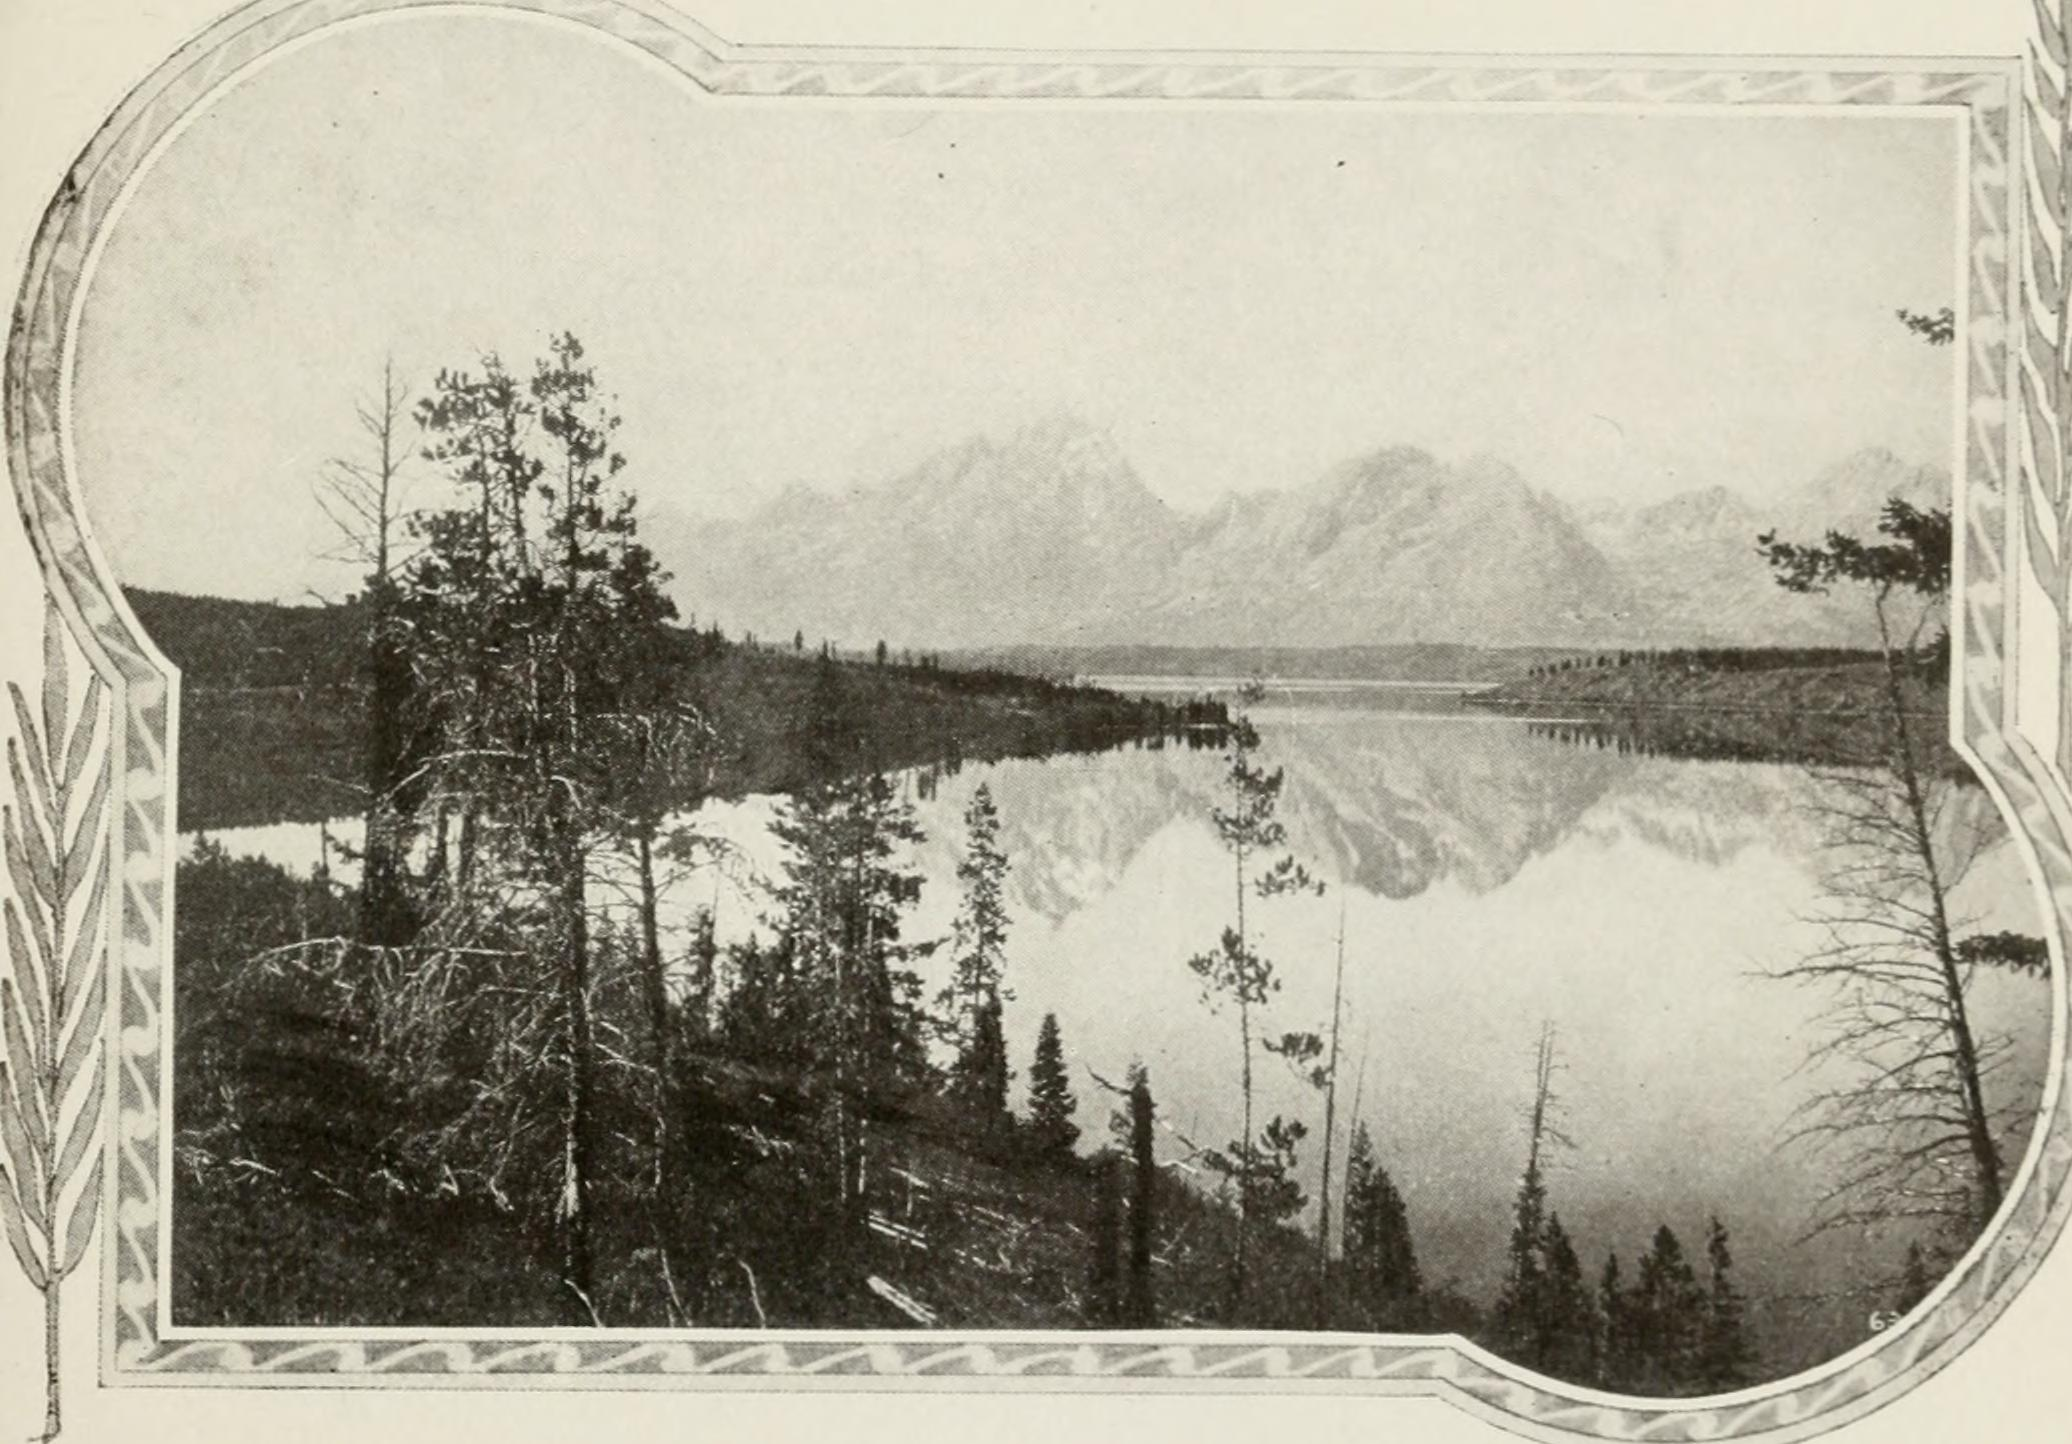
\includegraphics[width=\columnwidth]{geography-mountains}
}
\subsection*{Moutain Ranges}

Moutain ranges host a variety of life adjusted to the terrain and elevation. Small animals live amongst the many cracks and crevices, attracting bigger preadators. Verdant fields may span valleys between peaks, and caves in the mountains may stretch much deeper than at first glance. \\

Mountains are naturally a defensive geographical feature due to the difficult terrain. Transport through mountainous regions is slow and is often restricted to passes and paths. As a result, defensive human structures can be more common. \\

Consider the ecological and societal makeup in your montane regions.

\begin{itemize}
\item What larger monsters or beasts have come to pick off even the largest of mundane predators? How are they ajusted for a higher-altitude lifestyle?
\item What intelligent factions have taken up isolated residence among the peaks and valleys? Why have they decided to isolate themselves? How do they live in such an isolated environment?
\item What old structures remain in the mountains? Where do they lie among them?
\end{itemize}

Consider why a party of adventurous characters would visit such a place.

\begin{itemize}
\item Are there old ruins that might hide treasure or secrets?
\item Are there particular NPCs that have value to the party?
\item Are there rare biological ingredients here needed by the party?
\end{itemize}



\subsection*{Taiga Forest}

Northern forests see much snow, and as a result are full of moisture in spring. This can cause a variety of environmental conditions, from deep forests to wetlands and lakes. Natural resources are generally plentiful here, and human settlements are common. \\

Consider a specific region in your taiga region.

\begin{itemize}
\item What is the ecological makeup of this region? What are its main geographical features?
\item What kinds of peoples live here? What technology do they have, what is their relationship with their environment, and what relationships do they have with other nearby peoples?
\item What natural resources are unique to this region? What types of society flourish in an area with as mild of a climate?
\end{itemize}

\subsection*{Polar Seas}

Interspersed equally by icebergs and islands, the northern seas see more activity than one would expect, though not all is friendly. \\

Raiders will board the few trade ships around and ransack local villages. There are many fishers at work in the region, both near the shore and farther out, but weather, beast, and cold withhold plentiful bounties on every cast. \\

What activities are present in your northern seas?

\begin{itemize}
\item Who do raiders and marauders attack? What other societies are present?
\item How do player characters perform seafaring? Are they previously experienced, or do they need to hire a boat?
\item What sea creatures would interact with the party away from land?
\end{itemize}

\subsection*{Polar Caps}

There are no known standing structures beyond the northern seas. Only the coldest of winds blow. Snowy landscapes stretch interminably. Only the most foul of beasts live here.

\begin{itemize}
\item How have creatures adapted to the polar day and night cycles?
\item What preparation is needed to venture into this region? How long could one survive?
\item What treasure lies here? How can it be accessed?
\end{itemize}

\section{Weather and Cold}

Retaining heat is of the utmost importance in all of the Reaches.
Some relevant system considerations have been mentioned already, and will be expanded here. \\

{\centering
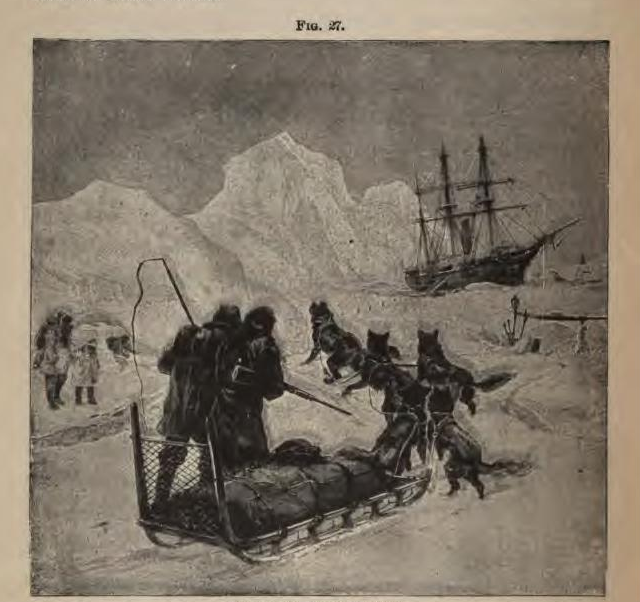
\includegraphics[width=\columnwidth]{arctic-sledders}
}

\subsection*{Weather Generation}

Weather is generated randomly for each period of 2 days. Roll d66 and consult the following table:

\begin{table*}[h]
  \centering
  \begin{tabular}{| c || c || c ||}
    \hline
    & Precipitation/Condition & Temperature/Air Quality \\ \hline
    1 & Clear and Bright & Frigid \\
    2 & Overcast & Cold \\
    3 & Lightly Snowfall & Humid \\
    4 & Heavy Snow & Biting Wind \\
    5 & Freezing Rain & Gale \\
    6 & Blizzard & Crisp  \\ \hline
  \end{tabular} \label{tbl:weather}
  \caption{Weather Generation Table}
  \label{tbl:weather}
\end{table*}  


\end{multicols}
\end{document}
